\definecolor{highlightcolor}{HTML}{d4dcf7}
\begin{table}[t]
\caption{
Main results for SWE-agent performance on the full and Lite splits of the SWE-bench test set.
We benchmark models in the SWE-agent, Basic CLI, and Retrieval Augmented Generation (RAG) settings established in SWE-bench~\citep{jimenez2024swebench}.
}
\label{table:main-results}
\vspace{0.25em}
\centering
\begin{tabular}{lcccc}
    \toprule
    & \multicolumn{2}{c}{SWE-bench} & \multicolumn{2}{c}{SWE-bench Lite} \\
    \cmidrule(lr){2-3} \cmidrule(lr){4-5}
    Model & \% Resolved & \$ Avg. Cost & \% Resolved & \$ Avg. Cost \\
    \cmidrule(lr){1-1} \cmidrule(lr){2-3} \cmidrule(lr){4-5}
    RAG                        &             &      &             &      \\
    \smalltab w/ GPT-4 Turbo   &       1.31  & 0.13 &       2.67  & 0.13 \\
    \smalltab w/ Claude 3 Opus &       3.79  & 0.25 &       4.33  & 0.25 \\
    \cmidrule(lr){1-1}
    Shell-only agent                   &     &      &             &      \\
    \smalltab w/ GPT-4 Turbo           & -   & -    &      11.00  & 1.46 \\
    \smalltab\smalltab w/o Demonstration & -   & -   
    &       7.33  & 0.79 \\
    \cmidrule(lr){1-1}
    SWE-agent                  &             &      &             &      \\
    \smalltab w/ GPT-4 Turbo   & {\bf 12.47} & 1.59 & {\bf 18.00} & 1.67 \\
    \smalltab w/ Claude 3 Opus &      10.46  & 2.59 &      13.00  & 2.18 \\
    \bottomrule
\end{tabular}
% \end{table}

% \begin{table}
\renewcommand{\arraystretch}{1.1} % Adjust this value as needed
\begin{minipage}[b]{0.6\textwidth}
\caption{Pass@1 results on HumanEvalFix~\cite{muennighoff2023octopack}. Except for SWE-agent, we use scores as reported in~\citet{yu2023wavecoder}.}
\label{tab.benchmark_humanevalfix}
\vspace{0.25em}
\centering
\begin{tabular}{lcccc}
\toprule
    Model & Python & JS & Java \\
\midrule
    CodeLLaMa-instruct-13B & 29.2 & 19.5 & 32.3\\
    GPT-4 & 47.0 & 48.2 & 50.0 \\
    \small DeepseekCoder-CodeAlpaca-6.7B & 49.4 & 51.8 & 45.1 \\
    WaveCoder-DS-6.7B & 57.9 & 52.4 & 57.3 \\
    SWE-agent w/ GPT-4 Turbo & \textbf{87.7} & \textbf{89.7} & \textbf{87.9} \\
\bottomrule
\end{tabular}
\end{minipage}
\hfill
\begin{minipage}[b]{0.38\textwidth}
    \centering
    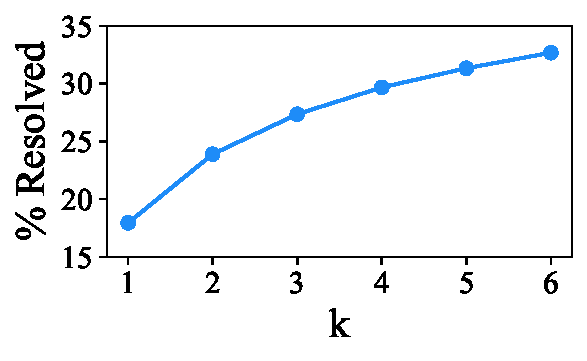
\includegraphics[width=\textwidth]{figures/pass_at_k.pdf}
    \captionof{figure}{
    SWE-agent w/ GPT-4 Turbo Pass$@k$ performance across \num{6} runs on SWE-bench Lite.
    }
    \label{fig:pass_at_k}
\end{minipage}

\centering
\caption{
SWE-bench Lite performance under ablations to the SWE-agent interface, which is denoted by \twemoji{cowboy_hat_face}. 
We consider different approaches to searching and editing (see Figures~\ref{fig.search.comparison} and \ref{fig.edit.comparison}, respectively).
We also verify how varying the file viewer window size affects performance, and we ablate the effect of different context management approaches.
}
\label{tab:combined_ablations_summary}
\vspace{0.25em}
{
\small
\begin{tabular}[t]{@{\hspace{0.05in}}l@{\hspace{0.07in}}l@{\hspace{0.05in}}}
    \toprule
    \multicolumn{2}{c}{\textbf{{Editor}}} \\
    \midrule
    \texttt{edit} action & 15.0  \decrease{3.0} \\
    \quad w/ linting \twemoji{cowboy_hat_face} & 18.0 \\
    No \texttt{edit} & 10.3 \decrease{7.7} \\
    \bottomrule
\end{tabular}
\hspace{0.05in}
\begin{tabular}[t]{@{\hspace{0.05in}}l@{\hspace{0.07in}}l@{\hspace{0.05in}}}
    \toprule
    \multicolumn{2}{c}{\textbf{{Search}}} \\
    \midrule
    Summarized \twemoji{cowboy_hat_face} & 18.0 \\
    Iterative & 12.0 \decrease{6.0} \\
    No search & 15.7 \decrease{2.3} \\
    \bottomrule
\end{tabular}
\hspace{0.05in}
\begin{tabular}[t]{@{\hspace{0.05in}}l@{\hspace{0.07in}}l@{\hspace{0.05in}}}
    \toprule
    \multicolumn{2}{c}{\textbf{{File Viewer}}} \\
    \midrule
    30 lines & 14.3 \decrease{3.7} \\
    100 lines \twemoji{cowboy_hat_face}  & 18.0 \\
    % 400 lines &  17.0 \decrease{1.0} \\
    Full file & 12.7 \decrease{5.3} \\
    \bottomrule
\end{tabular}
\hspace{0.05in}
\begin{tabular}[t]{@{\hspace{0.05in}}l@{\hspace{0.06in}}l@{\hspace{0.05in}}}
    \toprule
    \multicolumn{2}{c}{\textbf{{Context}}} \\
    \midrule
    Last 5 Obs. \twemoji{cowboy_hat_face}  & 18.0 \\
    Full history & 15.0 \decrease{3.0} \\
    w/o demo. & 16.3 \decrease{1.7} \\
    \bottomrule
\end{tabular}
}
\vspace{-3.5em}
\end{table}
